%! Author = Omar Iskandarani
%! Date = 2025-09-06

\documentclass[11pt]{article}

% Packages
\usepackage{amsmath,amssymb}
\usepackage{geometry}
\usepackage{graphicx}
\usepackage{hyperref}
\geometry{margin=1in}

% Macros (explicit, macro-free chat-safe)
\newcommand{\vswirl}{\mathbf{v}_{\!\boldsymbol{\circlearrowleft}}}
\newcommand{\SwirlClock}{S_t^{\boldsymbol{\circlearrowleft}}}
\newcommand{\rhoF}{\rho_{\!f}}
\newcommand{\GammaC}{\Gamma_C}
% --- Add to your preamble (if not already present) ---
%-------------------------------------------
% Put this in your preamble (once)
%-------------------------------------------
\usepackage{tikz}
\usetikzlibrary{calc,arrows.meta,decorations.markings,decorations.pathmorphing}

% A tiny style for loop arrows
\tikzset{
    looparrow/.style={-{Stealth[length=2.5mm,width=1.8mm]},thick},
    knotline/.style={ultra thick, blue!70},
    testloopON/.style={thick, draw=green!60!black},
    testloopOFF/.style={thick, draw=red!70},
    axes/.style={very thick, black},
}

\usepackage{siunitx}


% Styling helpers
\tikzset{
    axisline/.style={very thick, black},
    corecircle/.style={thick, dashed, gray},
    knotline/.style={ultra thick, blue!65},
    swirlarrow/.style={-{Stealth[length=3mm,width=2mm]}, thick},
    vline/.style={-{Stealth[length=3mm,width=2mm]}, thick, teal!70!black},
    tube/.style={line width=6pt, line cap=round},
    ghost/.style={opacity=0.25},
    labelbox/.style={fill=white, inner sep=2pt, rounded corners=2pt},
}

\usetikzlibrary{knots,hobby,calc,intersections,decorations.pathreplacing,shapes.geometric,spath3}

% ------- Shared styles (from your preamble) -------
\tikzset{
    knot diagram/every strand/.append style={ultra thick, black},
%    every path/.style={black,line width=2pt},
%    every node/.style={transform shape,knot crossing,inner sep=1.5pt},
%    every knot/.style={line cap=round,line join=round,very thick},
%    strand/.style={line cap=round,line join=round,line width=3pt,draw=black},
%    over/.style={preaction={draw=white,line width=6.5pt}},
%    sst/ring A/.style={draw=black, line width=3pt},
%    sst/ring B/.style={draw=black,  line width=3pt},
%    sst/ring C/.style={draw=black, line width=3pt},
}

% ------- Guides toggle -------
\newif\ifsstguides
\sstguidestrue

% ------- Helper: label & skeleton for points P1..Pn -------
\newcommand{\SSTGuidesPoints}[2]{% #1=basename (e.g. P), #2=last index
    \ifsstguides
    \foreach \i in {1,...,#2}{
        \fill[blue] (#1\i) circle (1.2pt);
        \node[blue,font=\scriptsize,above] at (#1\i) {\i};
    }
    \draw[gray!40, dashed] \foreach \i [remember=\i as \lasti (initially 1)] in {2,...,#2,1} { (#1\lasti)--(#1\i) };
    \fi
}

\begin{document}

\title{Long-Distance Swirl Gravity from Chiral Swirling Knots with Central Holes}
\author{Omar Iskandarani}
\date{\today}
\maketitle

\begin{abstract}
We derive long-range gravitational attraction in Swirl--String Theory (SST) as a direct consequence of \emph{chiral swirling knots}---topological vortex filaments such as the trefoil ($3_1$), cinquefoil ($5_1$, $5_2$), and stevedore ($6_1$).
Each knot encloses a central rotational line, which acts as an anchor of circulation.
Using Cauchy's integral theorem, we show that the circulation measured around any loop enclosing this axis is quantized by the knot's winding number.
This quantization is expressed by the Swirl Clock $\SwirlClock$, and its persistence explains why neutral molecules (e.g.\ H$_2$) attract in otherwise flat space: their knots are connected via the same central swirl line extending beyond the equal-pressure boundary.
\end{abstract}



% ====================================================================
% LATEX SWIRL STRING THEORY
% KNOT LIBRARY
% ====================================================================

\begin{table}[htbp]
\centering
\begin{tabular}{|ll|}
\toprule

% ====================================================================
% 6_1: Down Quarck Stevedore
% Usage: \SSTdown
% ====================================================================

        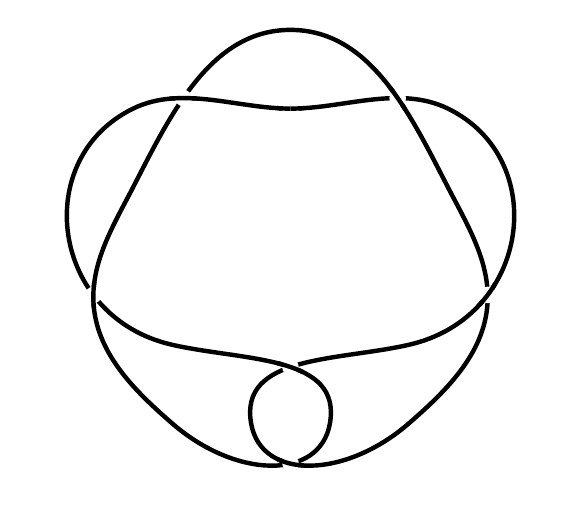
\begin{tikzpicture}[use Hobby shortcut]
        \coordinate (P1)  at ( 0,  2);
        \coordinate (P2)  at (-2,  2);
        \coordinate (P3)  at (-1.5, -1);
        \coordinate (P4)  at ( 0.5, -2);
        \coordinate (P5)  at (-1.5,-2);
        \coordinate (P6)  at (-2.5,-0.5);
        \coordinate (P7)  at (-2, 1);
        \coordinate (P8)  at ( 0,  3);
        \coordinate (P9)  at ( 2, 1);
        \coordinate (P10) at ( 2.5,-0.5);
        \coordinate (P11) at ( 1.5,-2);
        \coordinate (P12) at (-0.5, -2);
        \coordinate (P13) at ( 1.5, -1);
        \coordinate (P14) at ( 2,  2);
        \coordinate (P15) at ( 0,  2); % = P1

        \begin{knot}[
            consider self intersections,
            clip width=5pt, clip radius=3pt,
            ignore endpoint intersections=false,
            flip crossing/.list={2,4,6,8,10,12}
        % draft mode=crossings % uncomment to see numbers
        ]
        \strand
        ([closed] P1)..(P2)..(P3)..(P4)..(P5)..(P6)..(P7)..(P8)%
        ..(P9)..(P10)..(P11)..(P12)..(P13)..(P14)..(P15);
        \end{knot}
        \SSTGuidesPoints{P}{15}
        \end{tikzpicture}

&



% ====================================================================
% 5_2: Up Quark
% Usage: \SSTup
% ====================================================================

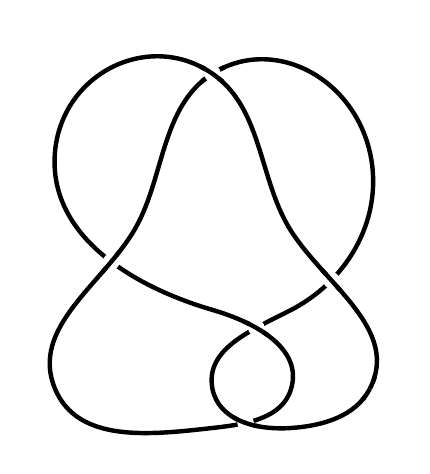
\begin{tikzpicture}[use Hobby shortcut]
\coordinate (P1) at (2, -2);
\coordinate (P2) at (1, 0);
\coordinate (P3) at (0, 2);
\coordinate (P4) at (-2, 1);
\coordinate (P5) at (0, -1);
\coordinate (P6) at (1, -2);
\coordinate (P7) at (0, -2.5);
\coordinate (P8) at (-2, -2);
\coordinate (P9) at (-1, 0);
\coordinate (P10) at (0, 2);
\coordinate (P11) at (2, 1);
\coordinate (P12) at (1, -1);
\coordinate (P13) at (0, -2);
\coordinate (P14) at (1, -2.5);
\coordinate (P15) at (2, -2); % = P1

\begin{knot}[
    consider self intersections,
    clip width=5pt, clip radius=3pt,
    ignore endpoint intersections=false,
    flip crossing/.list={2,4,6,8,10,12,14,16,18}
% draft mode=crossings
]
\strand
([closed] P1)..(P2)..(P3)..(P4)..(P5)..(P6)..(P7)..(P8)..(P9)..(P10)..(P11)..(P12)..(P13)..(P14)..(P15);
\end{knot}
\SSTGuidesPoints{P}{15}
\end{tikzpicture}



\\
\bottomrule
\end{tabular}
\end{table}

\section{Chiral Swirling Knots and Central Holes}
    Consider a chiral knot $K$ embedded in $\mathbb{R}^3$, such as:
    \[
        3_1 \ (\text{trefoil}), \quad
        5_1 \ (\text{cinquefoil torus}), \quad
        5_2 \ (\text{cinquefoil twist}), \quad
        6_1 \ (\text{stevedore}).
    \]
    Each knot can be parametrized on a torus with major radius $R$ and minor radius $r$.
    The core tube of radius $r_c$ supports a tangential swirl velocity $\vswirl$, defining the \emph{Swirl Clock} $\SwirlClock$.

    A defining feature is that all these knots possess a \emph{central hole} threaded by a straight axis (taken as the $z$-axis).
    This axis is the ``fabric line'' of flat space: it is the singularity in the analytic swirl potential.

\section{Cauchy Integral and Circulation Quantization}
    Let $C$ be a closed loop in the $x$--$y$ plane encircling the $z$-axis.
    By Cauchy's integral theorem, for an analytic swirl potential $W(z)=\Phi+i\Psi$,
    \begin{equation}
    \oint_C \vswirl \cdot d\mathbf{l} =
    \begin{cases}
    0, & \text{if no singularity inside,}\\[4pt]
    2\pi i\, \mathrm{Res}\!\left(\frac{dW}{dz}, z=0\right), & \text{if axis enclosed.}
    \end{cases}
    \end{equation}
    In SST, the residue corresponds to the circulation quantum
    \begin{equation}
    \kappa = 2\pi\, v_c\, r_c,
    \end{equation}
    where $v_c$ is the swirl speed at the core boundary $r_c$.

    If the knot winds around the axis $n$ times (its \emph{linking number}),
    \begin{equation}
    \GammaC = n \kappa.
    \end{equation}
    This is the Cauchy--Kelvin equivalence: long-distance swirl circulation is locked to integer multiples of $\kappa$ by topology.

\section{Composite Baryon Tubes}
    Inside baryons, three quark knots (e.g.\ $5_2$, $5_2$, $6_1$) meet at a Y-shaped junction, forming a single composite swirl tube.
    By Kelvin's theorem, circulation is additive:
    \begin{equation}
    \Gamma_{\rm baryon} = \Gamma_1 + \Gamma_2 + \Gamma_3
    = 3 \kappa.
    \end{equation}
    Since $\Gamma = 2\pi r_c v_\theta$, this means the effective swirl velocity is tripled:
    \begin{equation}
    v_{\theta,\rm eff} = \frac{\Gamma_{\rm baryon}}{2\pi r_c} = 3 v_c,
    \end{equation}
    while the core radius $r_c$ remains essentially unchanged.
    The baryon thus behaves as a single tube with three times the circulation and a deeper pressure well.

    \paragraph{Swirl Clock scaling.}
        The Swirl Clock relation becomes
        \begin{equation}
        dt_{\rm local} = dt_\infty \sqrt{1 - \frac{(3 v_c)^2}{c^2}},
        \end{equation}
        predicting a more pronounced local time dilation, consistent with the larger rest mass of baryons relative to single quark knots.

\section{Swirl Gravity and Molecular Attraction}
Two composite tubes (e.g.\ two protons) sharing the same central line produce a combined circulation
\[
    \Gamma_{\rm total} = (3 \kappa)_{\rm proton} + (3 \kappa)_{\rm proton} = 6 \kappa,
\]
which deepens the shared pressure well and yields a stronger long-range attraction.
This explains why neutral molecules (e.g.\ H$_2$) still attract in Euclidean space: their baryon cores are connected by the same central line, and the resulting swirl gravity follows directly from the additive circulation.

\section{Conclusion}
Long-distance gravitational attraction in SST is a manifestation of topological quantization: chiral knots with central holes enforce non-vanishing circulation residues along a central line.
When multiple quark knots merge into a baryon, their circulations add linearly, forming a single composite tube with $3\kappa$ circulation.
This mechanism predicts the correct baryonic mass scaling and provides a flat-space explanation for molecular attraction.


% ============================
% Figure 1: Trefoil + central axis + circulation loops
% ============================
\begin{figure}[t]
\centering
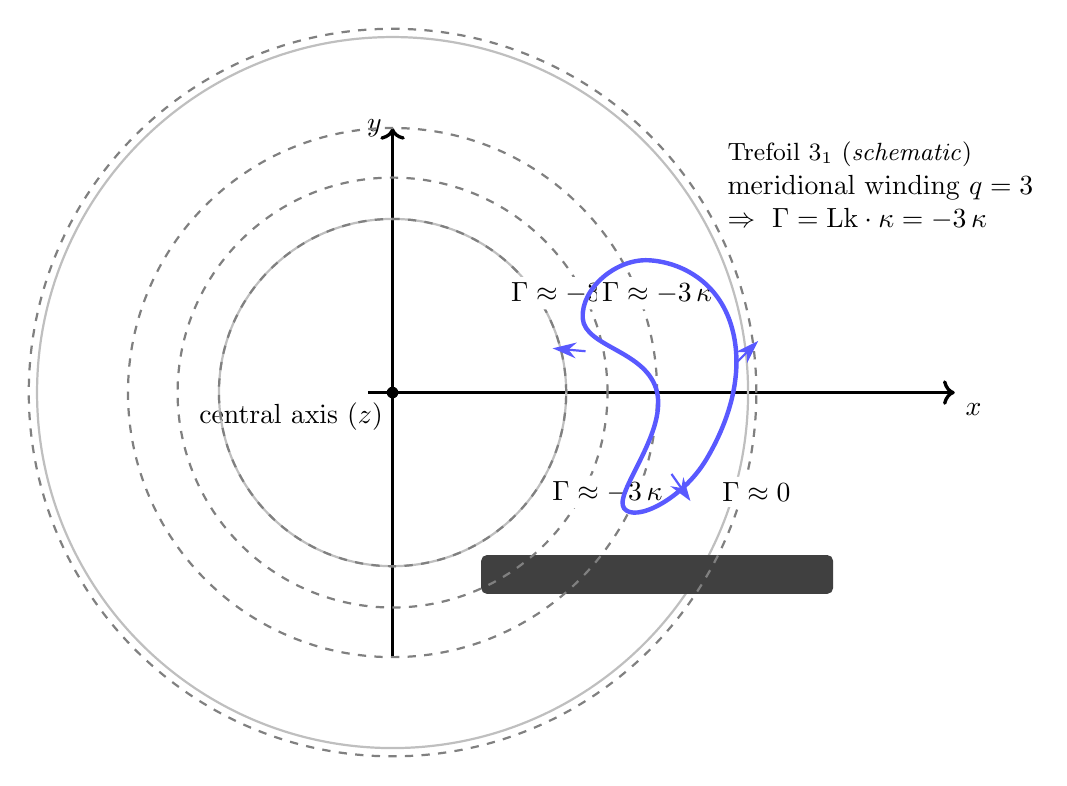
\begin{tikzpicture}[scale=1.05]
    % Parameters (schematic torus cross-section)
\def\R{3.2}   % major radius (to center of tube annulus)
\def\r{1.1}   % tube half-width in the drawing (annulus thickness/2)
\def\Rin{\R-\r}
\def\Rout{\R+\r}

% Coordinate axes (x-y plane view)
\draw[->,axisline] (-0.3,0) -- (6.8,0) node[below right] {$x$};
\draw[->,axisline] (0,-3.2) -- (0,3.2) node[left] {$y$};

% Central rotational axis (z-axis comes out-of-plane at (0,0))
\fill[black] (0,0) circle(2pt);
\node[below left] at (0,0) {central axis ($z$)};

% Annulus representing the torus "core circle" band (projection)
\draw[thick, gray!50] (0,0) circle (\Rin);
\draw[thick, gray!50] (0,0) circle (\Rout);
\node[labelbox,gray!50!black] at ({\R},-2.2) {torus annulus $[R-r,\,R+r]$};

% Circulation test loops (z=0 plane); inside annulus => plateau q=3
\foreach \RR in {2.1,2.6,3.2} {
    \draw[corecircle] (0,0) circle (\RR);
}
\node[labelbox] at (2.1,1.2) {$\Gamma \approx -3\,\kappa$};
\node[labelbox] at (2.6,-1.2) {$\Gamma \approx -3\,\kappa$};
\node[labelbox] at (3.2,1.2) {$\Gamma \approx -3\,\kappa$};

% Outside loop: ~0
\draw[corecircle] (0,0) circle (4.4);
\node[labelbox] at (4.4,-1.2) {$\Gamma \approx 0$};

% Schematic trefoil projection (simple stylized 3-lobe curve around core circle)
\begin{scope}
\draw[knotline]
plot[smooth cycle, tension=0.8]
coordinates {
    ({\R},0.0)
    ({\R-0.9},0.9)
    ({\R-0.1},1.6)
    ({\R+0.9},0.8)
    ({\R+0.6},-0.8)
    ({\R-0.4},-1.4)
};
% swirl direction arrows along the knot
\foreach \ang/\rad in {20/0.4,150/0.4,280/0.4}{
    \draw[swirlarrow, blue!65] ({\R+cos(\ang)*1.0},{sin(\ang)*1.0}) -- ++({cos(\ang+25)*\rad},{sin(\ang+25)*\rad});
}
\end{scope}

% Caption annotations
\node[align=left, labelbox] at (5.9,2.5) {%
    \small Trefoil $3_1$ (\emph{schematic})\\
    meridional winding $q=3$\\
    $\Rightarrow\ \Gamma=\mathrm{Lk}\cdot\kappa=-3\,\kappa$
};
\end{tikzpicture}
\caption{Trefoil knot with central axis and circulation loops in the $z{=}0$ plane.
Loops whose spanning disk intersects the filament within the torus annulus measure a constant plateau $\Gamma=\mathrm{Lk}\cdot\kappa=\pm 3\,\kappa$ (sign by orientation).
Loops outside the annulus do not enclose the filament and give $\Gamma\approx 0$.}
\label{fig:trefoil_axis_plateau}
\end{figure}

% ============================
% Figure 2: Baryon composite tube (Y-junction -> single tube)
% ============================
\begin{figure}[t]
\centering
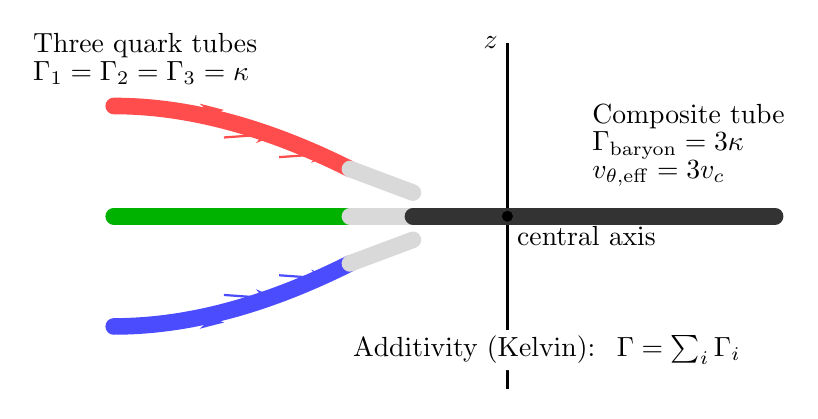
\begin{tikzpicture}[scale=1.0]
    % Central axis
\draw[axisline] (0,-2.2) -- (0,2.2);
\node[left] at (0,2.2) {$z$};

% Three incoming quark tubes (left side), colored
\draw[tube, red!70] (-5, 1.4) .. controls + (1,0) and +(-1,0.5) .. (-2, 0.6);
\draw[tube, green!70!black] (-5, 0.0) .. controls + (1,0) and +(-1,0.0) .. (-2, 0.0);
\draw[tube, blue!70] (-5,-1.4) .. controls + (1,0) and +(-1,-0.5) .. (-2,-0.6);

% Y-junction region
\draw[tube, gray!30,line cap=round] (-2,0.6) -- (-1.2,0.3);
\draw[tube, gray!30,line cap=round] (-2,0.0) -- (-1.2,0.0);
\draw[tube, gray!30,line cap=round] (-2,-0.6) -- (-1.2,-0.3);

% Merge into single composite tube (right side)
\draw[tube, black!80] (-1.2,0.0) .. controls +(0.8,0) and +(-0.8,0) .. (3.4,0.0);

% Swirl direction arrows on tubes
\foreach \x/\y in {-4.3/1.30, -3.6/1.00, -2.9/0.75}{
    \draw[vline, red!70] (\x,\y) -- ++(0.7,0.05);
}
\foreach \x/\y in {-4.3/0.00, -3.6/0.00, -2.9/0.00}{
    \draw[vline, green!70!black] (\x,\y) -- ++(0.7,0.00);
}
\foreach \x/\y in {-4.3/-1.30, -3.6/-1.00, -2.9/-0.75}{
    \draw[vline, blue!70] (\x,\y) -- ++(0.7,-0.05);
}
\foreach \x in {-0.8,0.2,1.2,2.2}{
    \draw[vline, black!80] (\x,0.0) -- ++(0.8,0.0);
}

% Labels
\node[align=left, labelbox] at (-4.6,2.0) {Three quark tubes\\[-2pt] $\Gamma_1=\Gamma_2=\Gamma_3=\kappa$};
\node[align=left, labelbox] at (2.3,0.9) {Composite tube\\[-2pt] $\Gamma_{\text{baryon}}=3\kappa$\\[-2pt] $v_{\theta,\mathrm{eff}}=3v_c$};
\node[align=left, labelbox] at (0.5,-1.7) {Additivity (Kelvin): $\ \Gamma=\sum_i \Gamma_i$};

% Central axis marker
\fill (0,0) circle (2pt);
\node[below right] at (0,0) {central axis};
\end{tikzpicture}
\caption{Baryon core as a \emph{composite swirl tube}: three quark tubes (left) merge via a Y-junction into a single tube (right).
Circulation adds linearly, $\Gamma_{\rm baryon}=3\kappa$, so the effective tangential swirl is $v_{\theta,\mathrm{eff}} = 3 v_c$ while the core radius remains $\approx r_c$.
The composite tube anchors to the same central axis, preserving the long-distance circulation residue.}
\label{fig:baryon_composite_tube}
\end{figure}



%-------------------------------------------
% 4-panel cartoon (same scale / same view)
%-------------------------------------------
\begin{figure}[t]
\centering

% -------- helper macro: one panel --------------
% args: #1 = loop radius, #2 = ON/OFF style, #3 = caption text under panel
\newcommand{\OnePanel}[3]{%
    \begin{tikzpicture}[x=1cm,y=1cm,scale=0.90]
    % parameters (shared across all panels)
    \def\R{3.2}   % major radius (center of torus band)
    \def\r{1.1}   % half-thickness of torus band
    \def\tilt{0.55}% yscale to hint 3D tilt of torus
    \def\RL{#1}   % test loop radius

    % axes (same in all panels)
    \draw[axes,->] (-0.25,0) -- (6.8,0) node[below right] {$x$};
    \draw[axes,->] (0,-3.0) -- (0,3.0) node[left] {$y$};

    % central axis marker (z coming out of page)
    \fill (0,0) circle(2pt);
    \node[below left] at (0,0) {\footnotesize central axis ($z$)};

    % --- torus "band" with a little 3D hint (tilted annulus) ---
    % outer and inner tilted ellipses (yscale = tilt)
    \begin{scope}[yscale=\tilt]
    \draw[very thick, gray!40] (0,0) circle (\R+\r);
    \draw[very thick, gray!40] (0,0) circle (\R-\r);
    % faint fill between ellipses for depth cue
    \path[fill=gray!10,draw=none] (0,0) circle (\R+\r);
    \clip (0,0) circle (\R+\r);
    \fill[white] (0,0) circle (\R-\r);
    \end{scope}

    % --- schematic trefoil projection with over/under cues ---
    % front arc (solid), back arc (dashed + lighter) to hint 3D crossing
    % This is a clean cartoon, not exact geometry.
    % Back (far) lobe:
    \draw[knotline, dashed, opacity=0.35]
    plot[smooth cycle, tension=0.9]
    coordinates {
        ({\R+0.2},  0.10)
        ({\R-0.4},  0.95)
        ({\R+0.6},  0.85)
        ({\R+0.3}, -0.9)
        ({\R-0.9}, -1.05)
    };
    % Front (near) lobe with arrows (swirl direction)
    \draw[knotline]
    plot[smooth cycle, tension=0.9]
    coordinates {
        ({\R},     0.00)
        ({\R-0.6}, 1.00)
        ({\R+0.8}, 0.80)
        ({\R+0.4},-1.00)
        ({\R-0.8},-1.20)
    };
    % flow arrows along the visible lobe
    \foreach \t/\L in {0/0.35, 60/0.35, 180/0.35}{
        \draw[looparrow, blue!70]
        ({\R+0.7*cos(\t)},{0.1+0.9*sin(\t)}) --
        ++({0.7*cos(\t+25)*\L},{0.7*sin(\t+25)*\L});
    }

% --- test loop (the circulation contour) ---
    \draw[#2] (0,0) circle (\RL);

    % panel caption (under)
    \node at (3.0,-2.7) {\small #3};
    \end{tikzpicture}%
}

% --------- lay out four panels on one row ----------
\OnePanel{0.55}{testloopOFF}{(a)\; very small loop $\Rightarrow\ \Gamma=0$}\hspace{0.9cm}
\OnePanel{2.65}{testloopON}{(b)\; inside torus band $\Rightarrow\ \Gamma=-3\,\kappa$}\hspace{0.9cm}
\OnePanel{3.25}{testloopON}{(c)\; still inside band $\Rightarrow\ \Gamma=-3\,\kappa$}\hspace{0.9cm}
\OnePanel{4.60}{testloopOFF}{(d)\; far outside $\Rightarrow\ \Gamma\approx 0$}

\caption{Four identical-scale, top-down panels. The gray tilted annulus hints at the torus where the trefoil lives (donut seen at an angle).
The blue curve is a schematic trefoil; dashed parts are “behind” (3D cue).
The green **test loops** (b,c) lie \emph{within} the torus band and measure the plateau \(\Gamma=\mathrm{Lk}\cdot\kappa=\pm 3\,\kappa\) (sign by orientation).
Red loops (a,d) do not link the filament \(\Rightarrow \Gamma\approx 0\).}
\label{fig:fourpanel-3D-cartoon}
\end{figure}


\bibliographystyle{plain}
\bibliography{swirlgravity}






\end{document}
